\chapter{Fundamentação Teórica}
    Este capitulo busca contextualizar os principais conceitos abordados no presente trabalho, tais como os materiais utilizados como base e também a tecnologia adotada no desenvolvimento do projeto. E ao final, serão elencados alguns trabalhos correlatos.

    \section{ENEF}
        Com o intuito de fortalecer a conscientização financeira da população brasileira e promover a cidadania, foi instituída a Estratégia Nacional de Educação Financeira (ENEF). Esta estratégia abrange uma série de áreas de estudo, incluindo direitos, deveres, investimentos, previdência, poupança, crédito, seguros, consumo e planejamento financeiro. A amplitude de temas reflete o compromisso da ENEF em abranger todo o espectro de idade, desde o ambiente escolar até a fase adulta, por meio de abordagens pedagógicas adaptadas para cada estágio de desenvolvimento. O cerne das operações e planos de ação da ENEF repousa sobre seu plano diretor, o qual articula a importância fundamental desses conhecimentos para a construção de uma população financeiramente consciente. Este documento também delineia os cenários propícios para a implementação das ações planejadas.

        \subsection{Material Didático}
            Foram disponibilizados pela estratégia um total de 24 livros, onde 18 são destinados ao Ensino Fundamental e os outros 6 são para o Ensino Médio. Os livros são divididos em 12 para alunos e 12 para os professores, estes materiais têm o objetivo de transmitir os conteúdos propostos pela ENEF para os alunos durante sua vida escolar.

            Os livros do se iniciam no primeiro ano do Ensino Fundamental, com conceitos muito simples que vão moldando a cidadania das crianças, conceitos como planejamento e organização que são aplicados de forma prática para organização da sala de aula e de festas. O material também apresenta a origem de produtos comuns do dia a dia como batatas, leite e a bola. A partir do livro 3 começam a ser introduzidos conceitos financeiros básicos, sendo realizada uma introdução as contas domésticas, como elas são calculadas conforme o consumo de cada equipamento. Após isso tem-se o início da contextualização do dinheiro físico e como ele é feito e usado e por fim reciclado.

            No 5º e 6º livro temos uma dinâmica um pouco diferente, sendo a aplicação de alguns jogos no formato livro-jogo, que permite ao usuário tomar decisões que podem o levar por diferentes caminhos e finais, algumas das possibilidades estão demonstradas na Figura 1. As alternativas são disponibilizadas ao usuário ao final da leitura do cenário e podem conter duas ou três possibilidades de caminhos a seguir, conforme Figuras 2 e 3.

            Já nas fases finais do Ensino Fundamental são abordados conceitos e instituições que disponibilizam algum recurso para a sociedade, pontuando a atribuição de cada organização. São algumas das organizações estudadas: Banco, Agência de Viagens, Hotel, dentre outras.

            \begin{figure}[h]
                \centering
                \caption{Esquema com alguns dos caminhos possíveis da primeiro jogo/história.}
                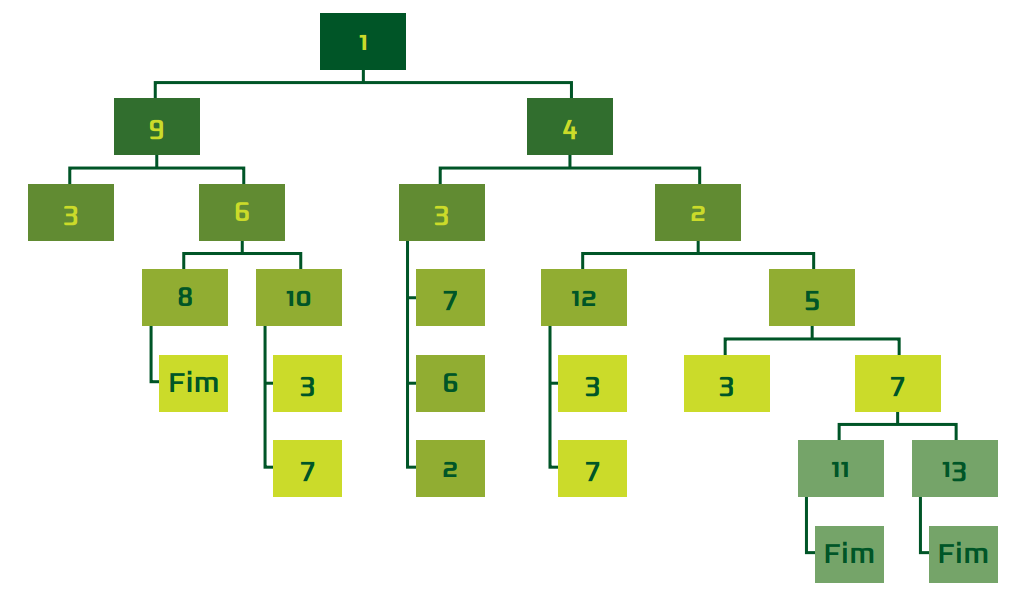
\includegraphics[scale=0.3]{Textuais/Pictures/Picture1.png}
                \fonte{\cite{Educacao_financeira_nas_escolas_professor}}\label{fig:figure-1}
            \end{figure}
            \begin{figure}[h]
                \centering
                \caption{Momento de decisão com duas possibilidades de caminhos.}
                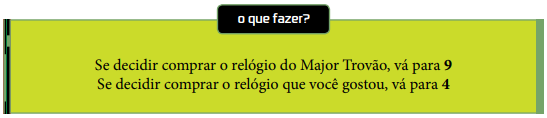
\includegraphics[scale=1]{Textuais/Pictures/Picture2.png}
                \fonte{\cite{Educacao_financeira_nas_escolas}}\label{fig:figure-2}
            \end{figure}
            \begin{figure}[h]
                \centering
                \caption{Momento de decisão com duas possibilidades de caminhos.}
                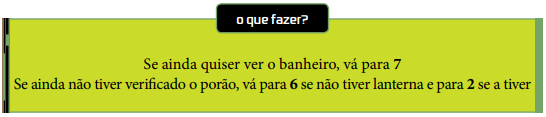
\includegraphics[scale=1]{Textuais/Pictures/Picture3.png}
                \fonte{\cite{Educacao_financeira_nas_escolas}}\label{fig:figure-3}
            \end{figure}
    
    \section{RPGJS}
         \textit{RPGJs} surge como um \textit{framework} inovador desenvolvido em TypeScript, destinado a simplificar a concepção e elaboração de jogos de interpretação de personagens (RPG). Este projeto de código aberto oferece um ambiente para a criação de jogos do gênero \textit{Role-Playing Game} (RPG) e \textit{Massively Multiplayer Online Role-Playing Game} (MMORPG), acessíveis diretamente por meio de navegadores web.

        Nos cenários construídos com o \textit{RPGJs}, os jogadores ganham vida em coordenadas distintas de um mapa, adaptando-se às demandas do enredo. O \textit{framework} incorpora elementos essenciais, como eventos e cenas, possibilitando aos jogadores a tomada de decisões ao longo da narrativa. Para enriquecer a imersão, a inclusão de trilhas sonoras de fundo é viabilizada. A dimensão visual dos jogos é construída por meio da sinergia entre \textit{Tilesets} e \textit{Spritesheets} \cite{Documentacao_RPGJs}.

        \textit{Tilesets} materializam-se como conjuntos de \textit{Tiles}, onde cada \textit{Tile} representa um componente de arte \textit{pixel art} na tela, convergindo para a construção dos cenários. A possibilidade de dispor cada \textit{Tile} de maneira aleatória no \textit{Tilemap} introduz variações no leiaute do ambiente virtual. Elementos cruciais como paletas de cores do jogo e da tela são concebidos a partir da imagem central do jogador. Esta abordagem eficaz viabiliza ambientes visuais multifacetados e dinâmicos, ao passo que mantém a flexibilidade de arranjo dos elementos. Em essência, \textit{Tilesets} foram pensados como ferramentas essenciais para os criadores de jogos, permitindo a elaboração de mundos cativantes e esteticamente agradáveis por meio do encaixe estratégico de componentes \textit{pixel art} \cite{borges2021desenvolvimento}.

        Complementando a funcionalidade dos \textit{Tilesets}, \textit{Spritesheets} emergem como coleções de elementos 2D que descrevem as movimentações possíveis para um personagem ou objeto no contexto do jogo. Este recurso ostenta um valor inestimável para os artistas que almejam conceber imagens dinâmicas valendo-se de ferramentas convencionais. Ao otimizar tanto os custos de produção quanto a simplicidade na geração de imagens de alta qualidade, \textit{Spritesheets} fomentam modificações na aparência e comportamento de um objeto por meio de variações de poses. A geração automática de poses intermediárias potencializa a eficiência do processo criativo. A harmonização entre \textit{Spritesheets} e \textit{Tilesets} capacita os desenvolvedores a criar experiências visuais enriquecedoras, enraizando maior interatividade e imersão no universo dos jogadores \cite{jones2013dynamic}.

        \begin{figure}[h]
            \centering
            \caption{Visão da ferramenta de edição de mapas.}
            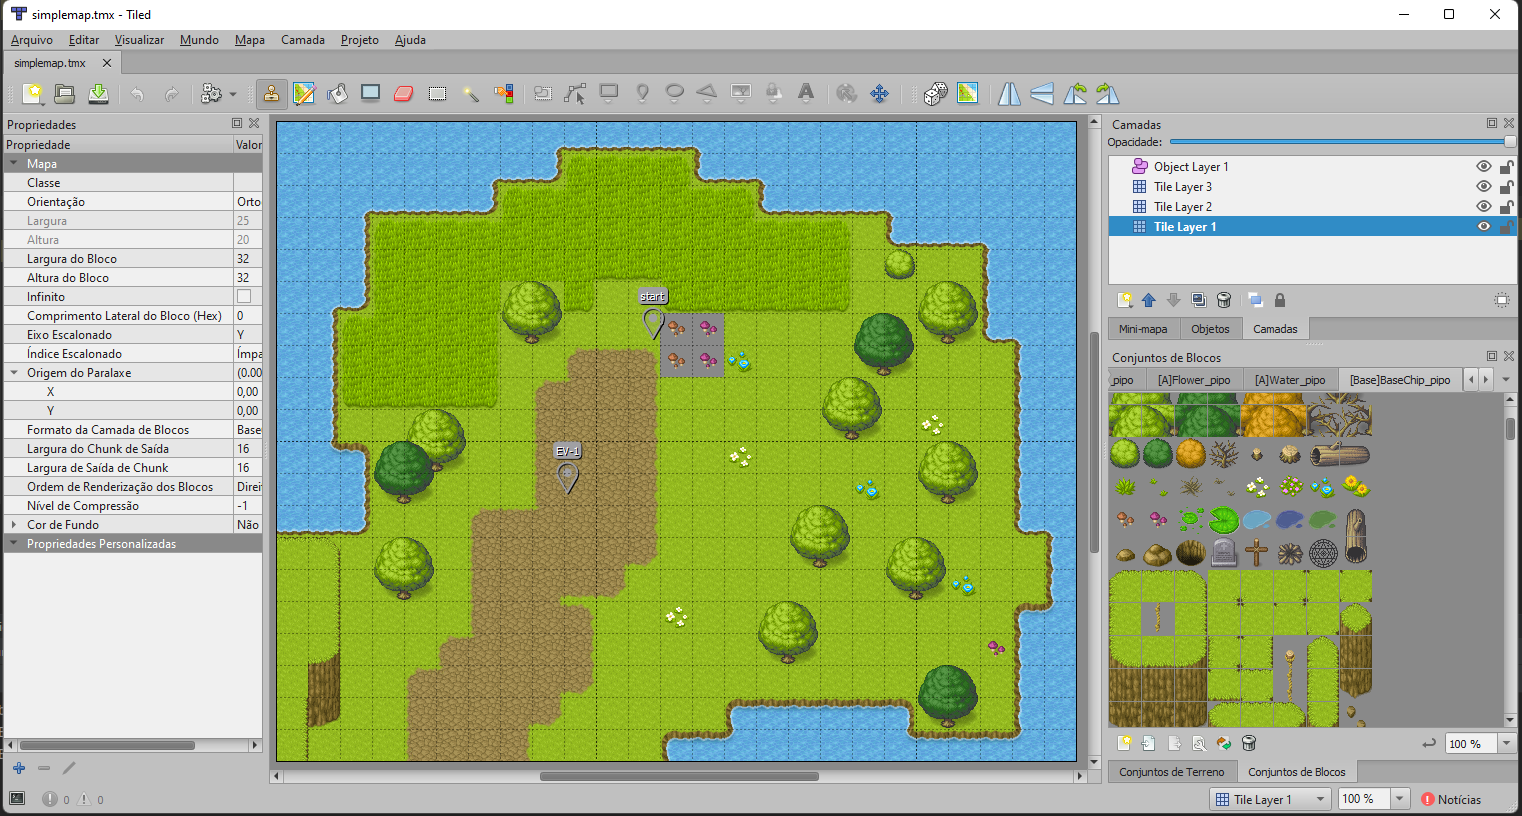
\includegraphics[scale=0.3]{Textuais/Pictures/Picture4.png}
            \fonte{\cite{Tiled}}\label{fig:figure-4}
        \end{figure}

        \begin{figure}[h]
            \centering
            \caption{\textit{Spritesheet.}}
            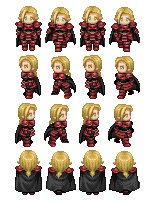
\includegraphics[scale=1.8]{Textuais/Pictures/Picture5.png}
            \fonte{\cite{Documentacao_RPGJs}}\label{fig:figure-5}
        \end{figure}


    \section{Trabalhos Correlatos}
        Nesta seção serão apresentados alguns trabalhos, que de alguma maneira se correlaciona com o presente trabalho.

        \subsection{Debt Maze}
            O \textit{Debt Maze}\cite{Debt_Maze} é um jogo projetado para ensinar conceitos financeiros de maneira envolvente. Com um labirinto repleto de desafios baseados em temas financeiros como empréstimos, juros e pagamentos em atraso, o jogo se adapta a jogadores de todos os níveis, desde novatos até os mais familiarizados com finanças. Navegar corretamente pelo labirinto é paralelo a tomar decisões financeiras acertadas na vida real. Integrando elementos imersivos, persuasivos e personalizáveis, \textit{Debt Maze}\cite{Debt_Maze} não somente entretém, mas também visa aprimorar a alfabetização financeira do jogador, equipando-o para tomar decisões mais informadas.

            Comparado ao \textit{Debt Maze}\cite{Debt_Maze}, que utiliza um labirinto para simbolizar os desafios financeiros, o presente trabalho adota uma abordagem mais prática e aplicável à vida cotidiana das crianças. Em vez de um jogo baseado em labirintos, o presente trabalho oferece cenários práticos e ferramentas para realizar escolhas financeiras reais, tornando o aprendizado mais direto.

        \subsection{PlanCash}
            O \textit{PlanCash}\cite{mariano2020educaccao} é um jogo de tabuleiro inovador, projetado para combinar aprendizado e diversão para o público infantil. Ele incorpora conteúdos convencionais de matemática e situações cotidianas, abordando tópicos como história do dinheiro, gestão financeira, economia e operações matemáticas básicas. Por meio de caminhos alternativos no tabuleiro, os jogadores são desafiados por cartas que propõem situações-problema, gerando reflexão e análise sobre cada proposta. As cartas, classificadas como Pergunta, Pagar, Receber, Recompensa e Roleta, oferecem uma dinâmica envolvente, onde as decisões dos jogadores influenciam seu progresso. Uma ferramenta educativa e lúdica, o \textit{PlanCash}\cite{mariano2020educaccao} é uma adição valiosa para o ensino fundamental e para famílias que buscam uma maneira divertida de ensinar conceitos financeiros e matemáticos às crianças.

            O \textit{PlanCash}\cite{mariano2020educaccao} oferece uma proposta lúdica por meio de um jogo de tabuleiro, combinando educação e entretenimento para crianças. No  entanto, o presente trabalho busca evoluir esse conceito, apresentando um formato digital, que é naturalmente mais atraente para a geração atual de crianças. A digitalização não apenas moderniza a proposta, mas também incorpora elementos visuais e interativos que ampliam a experiência educacional, tornando o aprendizado sobre finanças e matemática ainda mais envolvente.            

        \subsection{Finance Game}
            O \textit{Finance Game}\cite{Finance_Game}, desenvolvido como ferramenta educacional, aborda a gestão financeira de forma lúdica e interativa, buscando conscientizar os jogadores sobre a importância do equilíbrio entre a tomada de decisões financeiras e outros aspectos que impactam a qualidade de vida. Introduzindo os jogadores a cenários simulados da vida de um trabalhador adulto, como a administração de um orçamento pessoal e as implicações de escolhas de consumo, o jogo promove a reflexão sobre responsabilidade financeira e a busca por satisfação pessoal. Via interações com diversos elementos, como o mercado, banco e lanchonete, os jogadores são desafiados a tomar decisões que influenciam diretamente a sua situação econômica e bem-estar. O jogo visa a capacitar os jogadores a compreender as consequências de suas ações financeiras, incentivando a tomada de decisões informadas e ponderadas no mundo real.
            
            Ao comparar o \textit{Finance Game}\cite{Finance_Game} com o presente trabalho, destaca-se que a abordagem escolhida busca proporcionar uma imersão mais profunda ao contextualizar situações financeiras na realidade da criança. Isso cria uma conexão direta com suas experiências, permitindo decisões mais identificáveis e uma compreensão prática dos princípios de educação financeira.

        \subsection{InvestPlay}            
            O \textit{InvestPlay}\cite{santos2020investplay} é um jogo educacional que ensina educação financeira de maneira dinâmica. Os jogadores movem um personagem por casas, respondendo perguntas e tomando decisões sobre gastos e investimentos. O objetivo é equilibrar ativos e passivos, aprendendo sobre finanças. A jogabilidade é elogiada, mas o nível de algumas perguntas é desafiador para crianças. O jogo oferece personalização para diferentes temas educativos.           

            O \textit{InvestPlay}\cite{santos2020investplay} se destaca por sua abordagem educativa em finanças. Contudo, o presente trabalho, fundamentado na literatura da ENEF, busca refinar essa proposta. Direcionando o conteúdo especificamente para o entendimento infantil, propomos uma abordagem que simplifica conceitos, tornando-os mais acessíveis e pertinentes ao público infantil. Assim, a intenção é que as crianças assimilem os conceitos financeiros de maneira mais eficaz e contextualizada.

        \subsection{Considerações sobre os Trabalhos Correlatos}

            A seção de trabalhos correlatos apresenta uma variedade de abordagens utilizadas para educar e capacitar indivíduos no domínio financeiro. O exemplo do \textit{Debt Maze} ilustra a eficácia de usar mecânicas de jogos para tornar o aprendizado de conceitos financeiros mais envolvente e compreensível. Navegar por um labirinto, por exemplo, pode simbolizar os desafios financeiros e decisões que as pessoas enfrentam na vida real. A integração de elementos imersivos e persuasivos nos jogos não apenas entretém, mas também tem o potencial de aprimorar significativamente a alfabetização financeira do jogador.

Através da análise destes trabalhos, fica evidente que a gamificação é uma ferramenta poderosa para educar e capacitar as pessoas a tomar decisões financeiras mais informadas. No entanto, cada jogo ou abordagem tem suas particularidades, e a eficácia de cada um pode variar com base no público-alvo e nos objetivos de aprendizado pretendidos.








        \subsection{Considerações sobre os Trabalhos Correlatos}







Os trabalhos correlatos aqui analisados demonstram a ampla variedade de abordagens utilizadas para a educação financeira por meio de ferramentas lúdicas. A diversidade de estratégias, cenários, e sistemas de aprendizado evidencia a crescente necessidade de adaptar a instrução financeira aos diferentes públicos-alvo e contextos de vida. O jogo, como meio interativo, apresenta-se como um instrumento poderoso para tal tarefa.

O \textit{Finance Game} destaca-se pela sua abordagem prática ao retratar cenários financeiros que se alinham diretamente com as experiências cotidianas das crianças. Ao fazer isso, ele constrói uma ponte entre teoria e prática, permitindo que os jogadores absorvam conhecimentos de forma mais eficaz. O \textit{Debt Mazer}, por sua vez, utiliza um ambiente de labirinto para representar os desafios financeiros, enfatizando a importância da tomada de decisão informada, enquanto elementos de imersão e personalização intensificam a experiência educacional.